%%%%%%%%%%%%%%%%%%%%%%%%%%%%%%%%%%%%%%%%%%%%%%%%

% Specify the command that you want into the header of the
% index.md file

%%%%%%%%%%%%%%%%%%%%%%%%%%%%%%%%%%%%%%%%%%%%%%%%

% Options for packages loaded elsewhere
\PassOptionsToPackage{unicode}{hyperref}
\PassOptionsToPackage{hyphens}{url}
\PassOptionsToPackage{dvipsnames,svgnames*,x11names*}{xcolor}
%
\documentclass[
  12pt,
  oneside]{report}
%%\usepackage{lmodern}
%
% Set line spacing
\usepackage{setspace}
\setstretch{1.5}

\usepackage{amssymb,amsmath}
\usepackage{ifxetex,ifluatex}
\ifnum 0\ifxetex 1\fi\ifluatex 1\fi=0 % if pdftex
  \usepackage[T1]{fontenc}
  \usepackage[utf8]{inputenc}
  \usepackage{textcomp} % provide euro and other symbols
\else % if luatex or xetex
  \usepackage{unicode-math}
  \defaultfontfeatures{Scale=MatchLowercase}
  \defaultfontfeatures[\rmfamily]{Ligatures=TeX,Scale=1}
\fi
% Use upquote if available, for straight quotes in verbatim environments
\IfFileExists{upquote.sty}{\usepackage{upquote}}{}
\IfFileExists{microtype.sty}{% use microtype if available
  \usepackage[]{microtype}
  \UseMicrotypeSet[protrusion]{basicmath} % disable protrusion for tt fonts
}{}
\makeatletter
\@ifundefined{KOMAClassName}{% if non-KOMA class
  \IfFileExists{parskip.sty}{%
    \usepackage{parskip}
  }{% else
    \setlength{\parindent}{0pt}
    \setlength{\parskip}{6pt plus 2pt minus 1pt}}
}{% if KOMA class
  \KOMAoptions{parskip=half}}
\makeatother
\usepackage{xcolor}
\IfFileExists{xurl.sty}{\usepackage{xurl}}{} % add URL line breaks if available
\IfFileExists{bookmark.sty}{\usepackage{bookmark}}{\usepackage{hyperref}}
\hypersetup{
  pdfauthor={François Leroy, PhD student at CZU},
  colorlinks=true,
  linkcolor=Blue,
  filecolor=Blue,
  citecolor=Blue,
  urlcolor=Blue,
  pdfcreator={LaTeX via pandoc}}
\urlstyle{same} % disable monospaced font for URLs

%% Package geometry
\usepackage[left = 2cm,right = 2cm,top = 2cm,bottom = 2cm]{geometry}
\usepackage{pdflscape}


%\usepackage{longtable} % out of date, now in latex-tools package
\usepackage{booktabs}
% Correct order of tables after \paragraph or \subparagraph
\usepackage{etoolbox}
\makeatletter
\patchcmd\longtable{\par}{\if@noskipsec\mbox{}\fi\par}{}{}
\makeatother
% Allow footnotes in longtable head/foot
\IfFileExists{footnotehyper.sty}{\usepackage{footnotehyper}}{\usepackage{footnote}}
\makesavenoteenv{longtable}
\usepackage{graphicx}
\makeatletter
\def\maxwidth{\ifdim\Gin@nat@width>\linewidth\linewidth\else\Gin@nat@width\fi}
\def\maxheight{\ifdim\Gin@nat@height>\textheight\textheight\else\Gin@nat@height\fi}
\makeatother
% Scale images if necessary, so that they will not overflow the page
% margins by default, and it is still possible to overwrite the defaults
% using explicit options in \includegraphics[width, height, ...]{}
\setkeys{Gin}{width=\maxwidth,height=\maxheight,keepaspectratio}
% Set default figure placement to htbp
\makeatletter
\def\fps@figure{htbp}
\makeatother
\setlength{\emergencystretch}{3em} % prevent overfull lines
\providecommand{\tightlist}{%
  \setlength{\itemsep}{0pt}\setlength{\parskip}{0pt}}
\setcounter{secnumdepth}{5}
%%% Complete the preamble of the LaTeX template
%%%------------------------------------------------------------------------------

%% Bug de bookdown: ne traite plus la déclaration "otherlangs" dans le préambule
% Pour charger les langues, écriture ici en dur du produit de bookdown
% Corrigé le 22/11/2019. A retester régulièrement: supprimer ces lignes si la compilation fonctionne sans elles.
\usepackage{polyglossia}
  \setmainlanguage[variant=american]{english}
  \setotherlanguage[]{french}
% Bug persistant le 28/02/2020

% Advised with polyglossia and babel
\usepackage{csquotes}

% Environnement "Essentiel" en début de chapitre
\usepackage[tikz]{bclogo}
\newenvironment{Essentiel}
  {\begin{bclogo}[logo=\bctrombone, noborder=true, couleur=lightgray!50]{L'essentiel}\parindent0pt}
  {\end{bclogo}}

%% Package fontspec
\usepackage{fontspec}
\setmainfont{calibri}[
  Path           = ./fonts/,
  Extension      = .ttf,
  BoldFont       = calibrib,
  ItalicFont     = calibrili,
  BoldItalicFont = calibriz]

% Rename chapters
% Below, scrpit to prevent the "chapter n" and the space use for it to
% be displayed
\usepackage{titlesec}
\titleformat{\chapter}   
{\Huge}{\thechapter{. }}{0pt}{\Huge}
%{\thechapter{. }}
\titlespacing*{\chapter}{0pt}{-50pt}{10pt}
% -50 is to up the title and 10 is the space with the text below


% When using the natbib biblio package, includes "References" in the table of contents
\usepackage[nottoc]{tocbibind}

% To make the table caption full page width
\usepackage{caption}

% Make the figure float
\usepackage{float}
\usepackage{float}
\usepackage{booktabs}
\usepackage{longtable}
\usepackage{array}
\usepackage{multirow}
\usepackage{wrapfig}
\usepackage{colortbl}
\usepackage{pdflscape}
\usepackage{tabu}
\usepackage{threeparttable}
\usepackage{threeparttablex}
\usepackage[normalem]{ulem}
\usepackage{makecell}
\usepackage{xcolor}
\ifluatex
  \usepackage{selnolig}  % disable illegal ligatures
\fi
\usepackage[style=apa,]{biblatex}
\addbibresource{references.bib}

\author{François Leroy, PhD student at CZU}
\date{2021-09-17}

% to include pdf
\usepackage{pdfpages}



%%%%%%%%%%%%%%%%%%%%%%%%%%%%%%%%%%%%%%%%%%%%%%%%%%%%%%%%%%%%%
% Start of the documents
\begin{document}

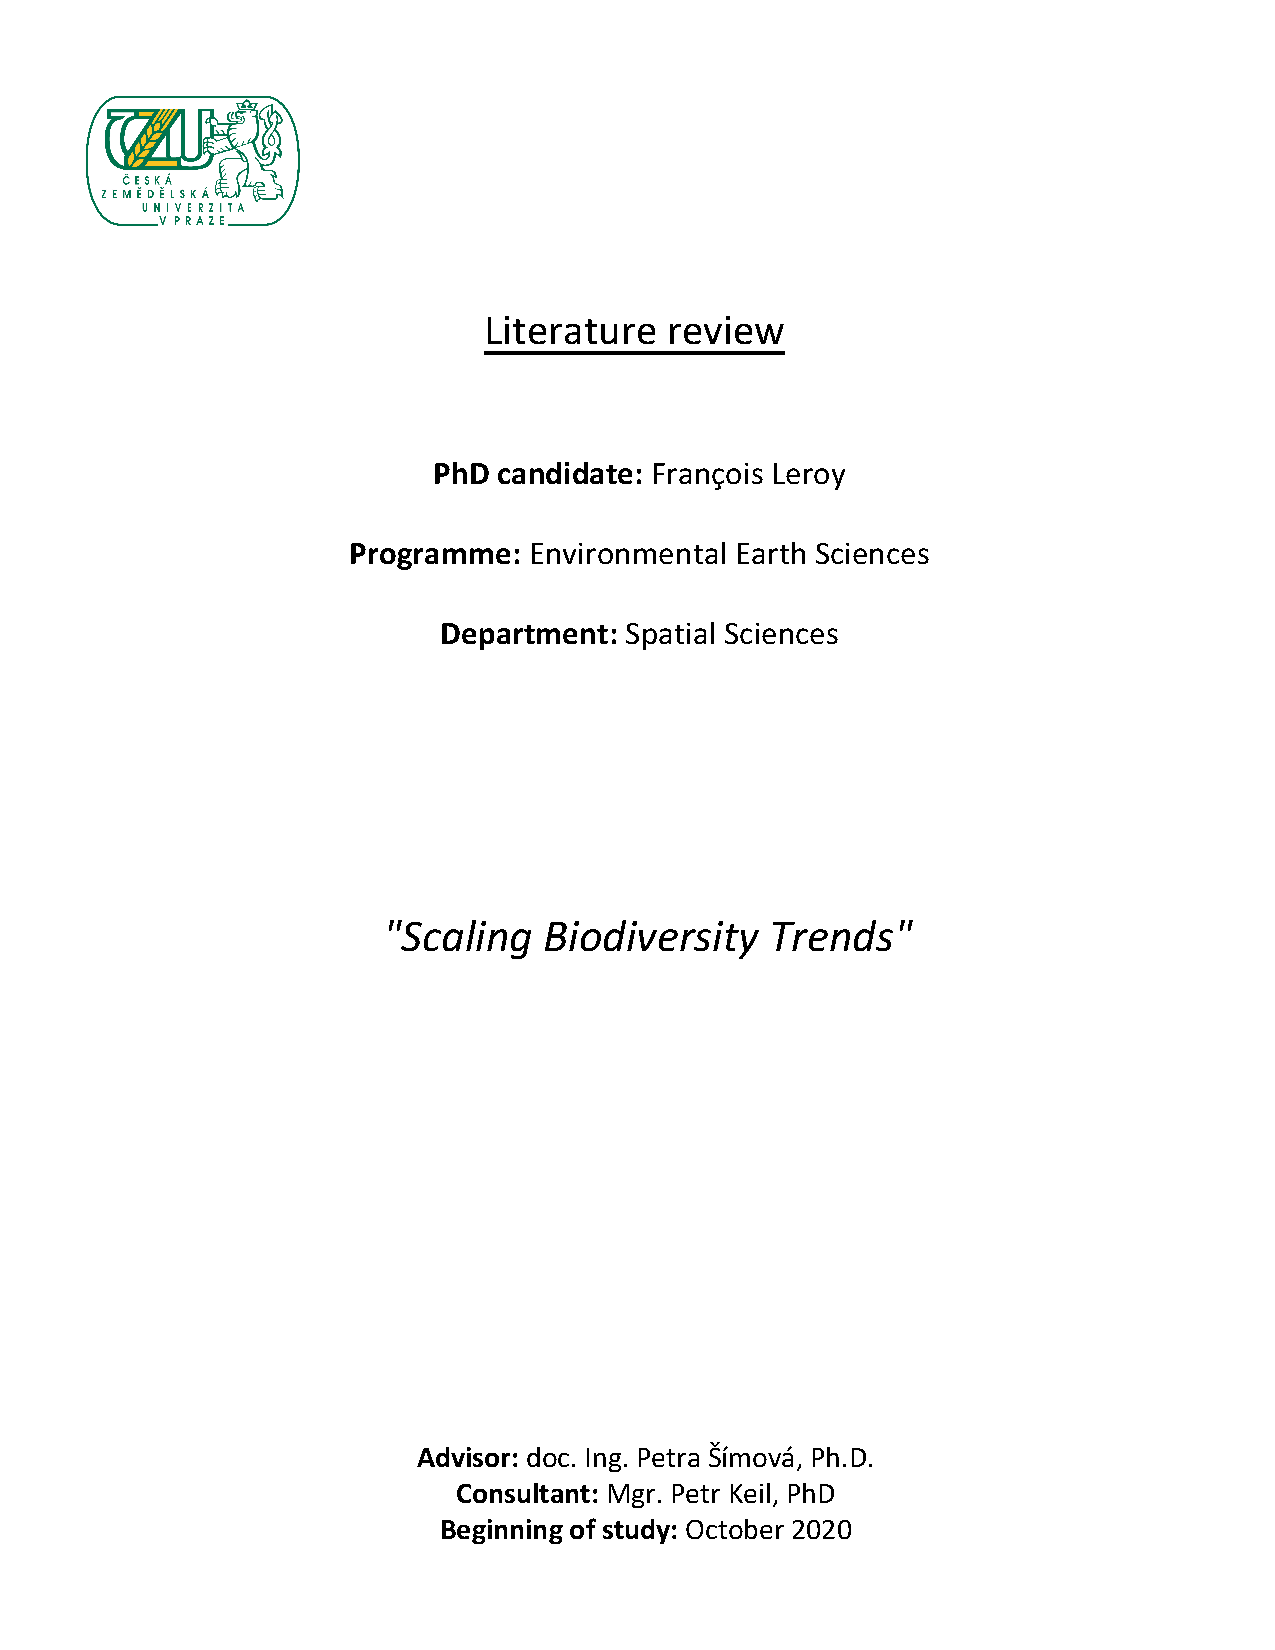
\includepdf[pages = {1}, fitpaper=true]{_assets/coverpage.pdf}

% Roman numbering for content before toc and toc itself
\cleardoublepage 
\pagenumbering{roman}

{
\hypersetup{linkcolor=}
\setcounter{tocdepth}{1}
\tableofcontents
\newpage
}
\vspace{50mm}
\setstretch{1.5}


% Start the arabic numbering at the 1st chapter
\cleardoublepage 
\pagenumbering{arabic}


% The mind, the...
\hypertarget{introduction}{%
\chapter{Introduction}\label{introduction}}

Human life quality is intrinsically linked to ecosystems state that he is living in. Indeed, ecosystems services extend in a large spectrum of mechanisms including nutrient cycle, food production, or climate and water cycle regulation \autocite{pereira_global_2012}. Some of those ecosystem functions are managed by bird biodiversity such as seed dispersal, controls pests or pollinate plant. Unfortunately, anthropogenic stressors like habitat loss, over exploitation, pollution or introduction of invasive species could lead biodiversity to its sixth mass extinction \autocite{barnosky_has_2011}.

We now know that the loss of global biodiversity is unprecedented and political decisions has been stated in order to limit it \autocite[\emph{e.g.}][2010, 2002]{secretariat_of_the_convention_on_biological_diversity_global_2006}. However, current scientific literature has also shown that temporal trends in local changes of biodiversity can be opposite to trends at larger scales \autocite[\emph{e.g.}][]{chase_species_2019}. Thus, current changes in biodiversity is far more complex than a simple global decrease: most of the ecosystems undergo alterations of their communities with changes in species composition \autocite{blowes_geography_2019,dornelas_quantifying_2013}. Wonders persist about how the trend of these different metrics of biodiversity are link to the spatial and temporal scales used when measured.

In order to investigate this link between spatio-temporal scales and biodiversity metrics, birds is a relevant taxon. Thanks to the many ornithological monitoring and surveys, we now have a large number of long, high-quality time series on bird populations \autocites{bejcek_velke_2016}{sauer_north_2013}{kamp_population_2021}. Birds are easy to observe, easy to identify and thus many volunteers are motivated to conduct standardized sampling. Given their ability to change quickly of locations, their presence is also a good indicator for ecosystem health and thus several standardized metrics have been created to assess their populations.

However, studying biodiversity can be confusing, especially because several choices must be done. Firstly, the level at which you are looking at the biodiversity must be chosen (\emph{e.g.} taxonomic, functional, phylogenetic diversity). Secondly, one must decide which metric is the most appropriate for his study. There are many facets of biodiversity that can be measured by different metrics depending on the objective of your study. Measures of static biodiversity are commonly used such as species richness or \(\alpha\) diversity \autocite[\emph{i.e.} number of species,][]{whittaker_vegetation_1960}, the Shannon index \autocite{shannon_mathematical_1948} ,the Simpson index \autocite{simpson_measurement_1949} or the Hill number \autocite{hill_diversity_1973}. The later three biodiversity indexes take into account the relative abundances of the species and can be considered as the \emph{quality} of the biodiversity. On an other hand, the spatial and temporal \(\beta\) diversity will measure the species turnover and can be measured thanks to Whittaker's \autocite{whittaker_evolution_1972}, Sørensen's \autocite{sorensen_method_1948} or Jaccard's \autocite{jaccard_distribution_1912} dissimilarity indexes \autocite[\emph{e.g.}][]{keil_patterns_2012}. All these metrics assess the taxonomic diversity, \emph{i.e.} they use the species as unit. However, it has also been shown that functional and phylogenetic diversity can provide supplementary information on the community structure and its dynamic \autocites[\emph{e.g.}][]{mcgill_rebuilding_2006}{mouquet_ecophylogenetics_2012}{webb_phylogenies_2002}.

An other measure of biodiversity of great interest is the abundance of the populations. As a matter of fact, as individuals react to disturbances of ecosystems by disappearing, the population trends are considered as resulting of the ecosystems health. Overall populations are impossible to assess, but determining the abundance of few indicator species can give a relevant summary on how is going the entire ecosystem \autocite{gregory_developing_2005}. These family of metrics are called the multi-species indicators (MSI) and we have seen the emergence of several of them according to the ecosystem considered. We can cite here the farmland bird indicator, woodland bird indicator or one of the most informative, which summarizes these two previous metrics: the Wildland Bird Indicator \autocite{gregory_generation_1999,gregory_wild_2010}. The main idea of these metrics is to compute the geometric mean of abundance of few key species over time.

Finally a last class of indicators, not considered here, take into account both species and ecosystems feature into a summarizing index. The most known ones are the Red List Index \autocite{butchart_improvements_2007,butchart_using_2005,butchart_measuring_2004} or the Biodiversity Change Index \autocite{normander_indicator_2012}.

Here, I propose to review articles assessing the temporal trends of different avian biodiversity metrics and to look at which spatial scales these studies have been done. I decided to consider the most common indicators used to assess biodiversity, such as the diversity indexes (\emph{e.g.} species richness, functional diversity\ldots) or the abundance indexes. Summarizing the trends of these qualitative and/or quantitative avian biodiversity indexes along with their spatial and temporal scales will help to see more clearly how the trends of biodiversity are linked to spatio-temporal scales. It is also important to demonstrate that the information about the sampling plan (\emph{i.e.} spatial scale, time span, temporal scales etc) is not systematically indicated in the scientific literature and can bring confusion to the analysis and comparisons of their trends. I believe that this review can help to have a better overview of the current knowledge on the trend of biodiversity metrics of bird populations.

\textcolor{red}{specify that it is mainly for continental/coastal birds but no look at  islandic communities and change *Stable* to *No trend*}

\hypertarget{materials-and-methods}{%
\chapter{Materials and Methods}\label{materials-and-methods}}

For this review, articles of interest were the ones assessing temporal trends of the most common indicators (\emph{i.e.} metrics) of avian biodiversity and specifying spatial and temporal scales. For this, I used the \emph{\enquote{advanced search}} tool of the ISI Web of Science Core collection database with these four following queries:

\begin{enumerate}
\def\labelenumi{\arabic{enumi}.}
\item
  \texttt{AB\ =\ ((biodiversity\ OR\ species\ richness\ OR\ diversity)\ AND\ (temporal\ trend*\ OR\ dynamic*)\ AND\ (bird*\ OR\ avia*))} which resulted in 1346 references.
\item
  \texttt{AB\ =\ ((biodiversity\ change\ index)\ \ AND\ (bird*\ \ OR\ avia*)\ \ AND\ trend*)} which resulted in 60 references.
\item
  \texttt{AB\ =\ ((species\ richness)\ AND\ (bird*\ OR\ avia*)\ AND\ trend*)} which resulted in 313 references.
\item
  \texttt{ALL=(birds\ AND\ species\ richness\ AND\ temporal\ trend)} which resulted in 88 references.
\end{enumerate}

Alternatively, the articles which were often referred to in the relevant articles were also explored.

I decided to take into account only the articles for which there was spatial replicates, \emph{i.e.} where the trend of the metric was assessed at several locations with the same spatial grain (except for the \emph{global scale}, which can not have spatial replicate). With this replications, the trend reported is more reliable. For each query, the title and abstract of the articles were reviewed. When the temporal trend was explicitly specified (either visually or literally), the material and method part was read in order to collect the \emph{spatial grain} of the trend (\emph{i.e.} the area at which the trend is assessed), its \emph{temporal grain} (\emph{i.e.} the time span at which data have been gathered at one census session), the \emph{spatial extent} (\emph{i.e.} the entire area at which the study applies), the \emph{temporal extent} and the \emph{beginning and ending years} of the study as well as the \emph{general trend} of the metric (Tab. \ref{tab:maintable}).

Spatial grain sizes are discretized into four levels: \emph{local} \(<= 25\) \(Km^2\), \emph{regional} \(> 25\) \(Km²\), \emph{national} when an entire country is considered and \emph{global} at the worldwide scale.

Concerning the trend assessment, different papers contain the \emph{p-value} or directly specify the significant trend of the metric. However, a portion of papers gives only visual representations of the trend. For those, the standard error was used when displayed. For the very few only giving the trend, \textcolor{red}{the rule of thumb was applied}. Information can be found in the column \emph{Note} of the Tab. \ref{tab:notetable} of the supplementary material. Moreover, the final trend retained (\emph{i.e.} either \emph{Increase}, \emph{Stable} or \emph{Decrease}) doesn't reflect all the fluctuations of the metric through time but rather the difference between the starting and ending points.

I have found 33 references in which authors were both determining the temporal trend of a metric of interest and explicitly defining the grain size. However, only 17 of them are using spatial replicates and are thus relevant for this study (Tab. \ref{tab:maintable}). The classes of metric are: \emph{Species richness, Evenness, Abundance, Diversity, Temporal beta-diversity, Spatial beta-diversity, Functional diversity, Functional evenness, Functional richness}. Some of this classes contain several different indexes. This is the case for instance for the class \emph{Diversity}, which can be defined by either the Shannon or the Simpson index, or for the class \emph{Abundance} which contains various multi-species indicators.

\hypertarget{results}{%
\chapter{Results}\label{results}}

\hypertarget{on-the-spatial-scale}{%
\section{On the spatial scale}\label{on-the-spatial-scale}}

Out of 17 papers, 5 were located in North America and 12 in Europe. The median spatial extent of the data is \ensuremath{5.20475\times 10^{5}} \(Km^2\), with the smallest area of 1800 \(Km^2\) and the greatest representing the global emerged surface (\emph{i.e.} \ensuremath{1.4894\times 10^{8}} \(Km^2\)). Overall, there were 11 \emph{Decrease}, 31 \emph{Increase} and 14 \emph{Stable} reliable trends (\emph{i.e.} spatially replicated) across the literature, without consideration of any metric or spatial scales.

Local scales are more represented than the others and the number of papers decreases with the increasing spatial scale (Figure \ref{fig:barspatscale}). This is expected, as the spatial replications get more demanding in organization and resources as the grain size enlarges. The \emph{Increase} of the metrics seems to be dominating at smaller scales. On an other hand, the proportion of \emph{Decrease} is more important at regional scales than at local scales. At the global scale, no \emph{Increase} were found.

\begin{figure}
\centering
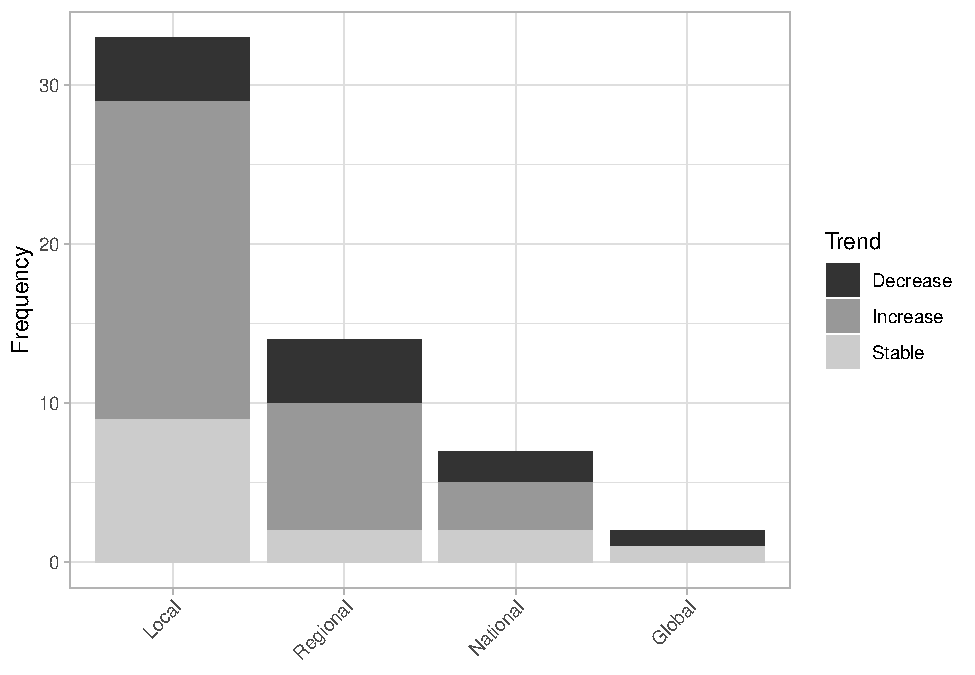
\includegraphics{literature_review_files/figure-latex/barspatscale-1.pdf}
\caption{\label{fig:barspatscale}Proportion of \emph{Increase}, \emph{Decrease} or \emph{Stable} trends for each spatial scale}
\end{figure}

Species richness and abundance metrics are very represented in the scientific literature (Figure \ref{fig:barmetrics}). The less common trend of abundance is \emph{Increase}, whilst \emph{Decrease} and \emph{Stability} are both as common. Diversity indexes (\emph{i.e.} Sørensen and Jaccard) were always found increasing and temporal \(\beta\)-diversity was found most of the time increasing and never decreasing. The small frequency of the other metrics doesn't allow one to discuss the trend proportions.

\begin{figure}
\centering
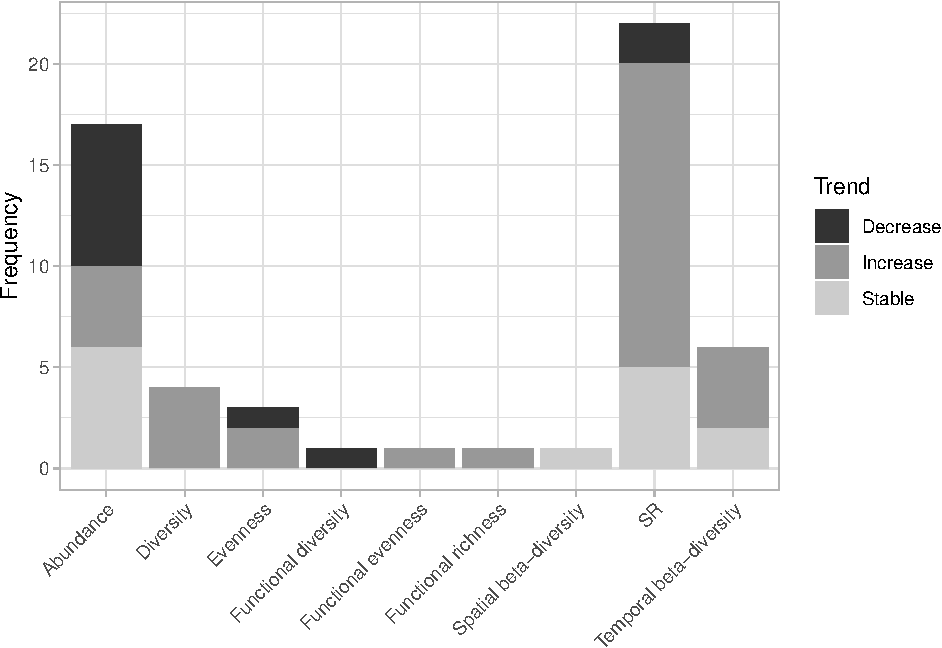
\includegraphics{literature_review_files/figure-latex/barmetrics-1.pdf}
\caption{\label{fig:barmetrics}Proportion of \emph{Increase}, \emph{Decrease} or \emph{Stable} trends for each of the metric}
\end{figure}

\textbf{At local scales}, species richness experiences dominantly increases (Figure \ref{fig:barmetricsperspatscale}). Evenness indexes, \emph{i.e.} taxonomic and functional evenness, are mainly found increasing. Concerning the abundance indexes, the stability dominates but the increase is also often witnessed. In contrast, \textbf{at regional scale}, abundance metrics always decrease, whilst temporal \(\beta\)-diversity always increase. Species richness experiments mainly increases, then stability but no decrease is reported. Concerning \textbf{national and global scales}, one have to keep in mind that spatial replicates are less frequent and that most of the trends reported here for these two spatial scales are not replicated. Exceptions are made by \textcite{bowler_geographic_2021} and \textcite{donald_agricultural_2001}. The former showed negative trends in abundance indexes for Denmark and Germany and positive trends for Switzerland and Czech Republic, indicating that one can not conclude about general trend at national scale (here referred as \emph{Stable}). For \textcite{donald_agricultural_2001}, trends of mean populations were computed for 30 european countries and most of them were negatives. No positive trend seem dominant at these spatial scales. Global trends only come from \textcite{jarzyna_taxonomic_2018}.

\begin{figure}
\centering
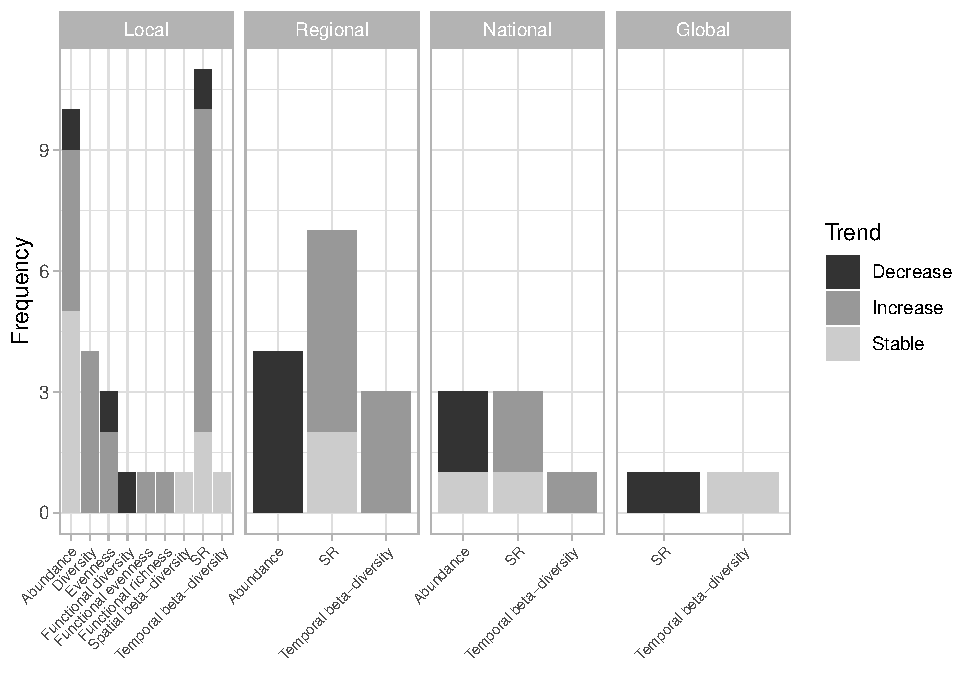
\includegraphics{literature_review_files/figure-latex/barmetricsperspatscale-1.pdf}
\caption{\label{fig:barmetricsperspatscale}Proportion of \emph{Increase}, \emph{Decrease} or \emph{Stable} trends for each metric. Each panel represent one spatial scale}
\end{figure}

\hypertarget{on-the-temporal-scale}{%
\section{On the temporal scale}\label{on-the-temporal-scale}}

The oldest study started in 1968 and the median duration is 23 years, with a minimum time span of 11 years and a maximum of 45.

\textbf{Don't know if the following part should be put in the discussion}

Determination of the temporal grain was way more complicated, as there is no consensus on the subject. Most of the time the temporal grain of the sampling was specified, but often with inaccuracies (\emph{e.g.} \enquote{in the early morning}). However, the temporal grain of the sampling plan doesn't represent the final temporal grain. For instance, some metrics are summed over a certain spatial extent \autocite[e.g.~summing the species richness over an atlas square, like in][]{van_turnhout_scale-dependent_2007}. In this case, the temporal grain should also be summed, but this was not specified. On an other hand, when the metric is averaged over a spatial grain, the sampling temporal grain can be considered.

However, an other problem arises when the trend is computed. Usually, one compute the metric out of the data and considers the value to be representative of half a year or a year. In this case, there is no consensus on what should be the temporal grain: should one keep the grain of the sampling? Should one consider it to be the time-span covered by the sampling?

For the cases where the metric was determined out of model \autocite[e.g.~][]{harrison_assessing_2014}, the final temporal grain was most of the time explicitly given, with an order of length of the year.

In short, temporal grain has no clear definition as it is different according to the metric computed, how it is computed and if the temporal trend is assessed. Even though it is now clear that sampling plan temporal grain is important to explicit, there is no such consensus regarding the temporal grain of the trend.

\begin{landscape}\begingroup\fontsize{10}{12}\selectfont

\begin{longtable}[t]{>{\raggedright\arraybackslash}p{6.5em}>{\raggedright\arraybackslash}p{6.5em}>{\raggedright\arraybackslash}p{6.5em}>{\raggedleft\arraybackslash}p{6.5em}>{\raggedleft\arraybackslash}p{6.5em}>{\raggedleft\arraybackslash}p{6.5em}>{\raggedright\arraybackslash}p{6.5em}>{\raggedright\arraybackslash}p{6.5em}>{\raggedright\arraybackslash}p{6.5em}}
\caption{\label{tab:maintable}Trends of different metrics of biodiversity at various spatial and temporal scales}\\
\toprule
Reference & Metric & Spatial grain (Km²) & Temporal grain (year) & Spatial extent (Km²) & Temporal extent (year) & Years & Country & Trend\\
\midrule
\endfirsthead
\caption[]{\label{tab:maintable}Trends of different metrics of biodiversity at various spatial and temporal scales \textit{(continued)}}\\
\toprule
Reference & Metric & Spatial grain (Km²) & Temporal grain (year) & Spatial extent (Km²) & Temporal extent (year) & Years & Country & Trend\\
\midrule
\endhead

\endfoot
\bottomrule
\endlastfoot
\cellcolor{gray!6}{\cite{barnagaud_temporal_2017}} & \cellcolor{gray!6}{Evenness} & \cellcolor{gray!6}{Local} & \cellcolor{gray!6}{1.0} & \cellcolor{gray!6}{9834000} & \cellcolor{gray!6}{41} & \cellcolor{gray!6}{1970-2011} & \cellcolor{gray!6}{USA} & \cellcolor{gray!6}{Increase}\\
 & SR & Local & 1.0 & 9834000 & 41 & 1970-2011 & USA & Increase\\
\cellcolor{gray!6}{\cite{bowler_geographic_2021}} & \cellcolor{gray!6}{Abundance} & \cellcolor{gray!6}{National} & \cellcolor{gray!6}{1.0} & \cellcolor{gray!6}{520475} & \cellcolor{gray!6}{27} & \cellcolor{gray!6}{1990-2016} & \cellcolor{gray!6}{Czech Rep., Switzerland, Denmark, Germany} & \cellcolor{gray!6}{Stable}\\
\cite{chase_species_2019} & SR & Local & 5.0 & 2800000 & 30 & 1982–2011 & USA, Canada & Stable\\
\cellcolor{gray!6}{} & \cellcolor{gray!6}{SR} & \cellcolor{gray!6}{Regional} & \cellcolor{gray!6}{5.0} & \cellcolor{gray!6}{2800000} & \cellcolor{gray!6}{30} & \cellcolor{gray!6}{1982–2011} & \cellcolor{gray!6}{USA, Canada} & \cellcolor{gray!6}{\vphantom{1} Stable}\\
\addlinespace
 & SR & Regional & 5.0 & 2800000 & 30 & 1982–2011 & USA, Canada & Stable\\
\cellcolor{gray!6}{} & \cellcolor{gray!6}{SR} & \cellcolor{gray!6}{Local} & \cellcolor{gray!6}{5.0} & \cellcolor{gray!6}{2800000} & \cellcolor{gray!6}{30} & \cellcolor{gray!6}{1982–2011} & \cellcolor{gray!6}{USA, Canada} & \cellcolor{gray!6}{\vphantom{1} Increase}\\
 & SR & Local & 5.0 & 2800000 & 30 & 1982–2011 & USA, Canada & Increase\\
\cite{chiron_forecasting_2013} & Abundance & Regional & 1.0 & 643801 & 14 & 2007-2020 & France & \vphantom{2} Decrease\\
\cellcolor{gray!6}{} & \cellcolor{gray!6}{Abundance} & \cellcolor{gray!6}{Regional} & \cellcolor{gray!6}{1.0} & \cellcolor{gray!6}{643801} & \cellcolor{gray!6}{14} & \cellcolor{gray!6}{2007-2020} & \cellcolor{gray!6}{France} & \cellcolor{gray!6}{\vphantom{1} Decrease}\\
\addlinespace
 & Abundance & Regional & 1.0 & 643801 & 14 & 2007-2020 & France & Decrease\\
 & Abundance & Regional & 1.0 & 643801 & 14 & 2007-2020 & France & Decrease\\
\cellcolor{gray!6}{\cite{davey_rise_2012}} & \cellcolor{gray!6}{Diversity} & \cellcolor{gray!6}{Local} & \cellcolor{gray!6}{1.0} & \cellcolor{gray!6}{242495} & \cellcolor{gray!6}{13} & \cellcolor{gray!6}{1994-2006} & \cellcolor{gray!6}{UK} & \cellcolor{gray!6}{Increase}\\
 & Evenness & Local & 1.0 & 242495 & 13 & 1994-2006 & UK & Increase\\
\cellcolor{gray!6}{} & \cellcolor{gray!6}{SR} & \cellcolor{gray!6}{Local} & \cellcolor{gray!6}{1.0} & \cellcolor{gray!6}{242495} & \cellcolor{gray!6}{13} & \cellcolor{gray!6}{1994-2006} & \cellcolor{gray!6}{UK} & \cellcolor{gray!6}{Increase}\\
\addlinespace
\cite{harrison_assessing_2014} & Abundance & Local & 1.0 & 200000 & 18 & 1994-2011 & Great Britain, UK & Increase\\
\cellcolor{gray!6}{} & \cellcolor{gray!6}{Abundance} & \cellcolor{gray!6}{Local} & \cellcolor{gray!6}{1.0} & \cellcolor{gray!6}{200000} & \cellcolor{gray!6}{18} & \cellcolor{gray!6}{1994-2011} & \cellcolor{gray!6}{Great Britain, UK} & \cellcolor{gray!6}{\vphantom{1} Stable}\\
 & Abundance & Local & 1.0 & 200000 & 18 & 1994-2011 & Great Britain, UK & Stable\\
\cellcolor{gray!6}{\cite{harrison_quantifying_2016}} & \cellcolor{gray!6}{Abundance} & \cellcolor{gray!6}{Local} & \cellcolor{gray!6}{0.5} & \cellcolor{gray!6}{242495} & \cellcolor{gray!6}{20} & \cellcolor{gray!6}{1994-2013} & \cellcolor{gray!6}{UK} & \cellcolor{gray!6}{Increase}\\
 & Abundance & Local & 0.5 & 242495 & 20 & 1994-2013 & UK & \vphantom{1} Stable\\
\addlinespace
\cellcolor{gray!6}{} & \cellcolor{gray!6}{Abundance} & \cellcolor{gray!6}{Local} & \cellcolor{gray!6}{0.5} & \cellcolor{gray!6}{242495} & \cellcolor{gray!6}{20} & \cellcolor{gray!6}{1994-2013} & \cellcolor{gray!6}{UK} & \cellcolor{gray!6}{Stable}\\
\cite{jarzyna_taxonomic_2018}\cellcolor{gray!6}{} & \cellcolor{gray!6}{SR} & \cellcolor{gray!6}{Regional} & \cellcolor{gray!6}{1.0} & \cellcolor{gray!6}{9834000} & \cellcolor{gray!6}{45} & \cellcolor{gray!6}{1969-2013} & \cellcolor{gray!6}{USA} & \cellcolor{gray!6}{\vphantom{1} Increase}\\
 & SR & Regional & 1.0 & 9834000 & 45 & 1969-2013 & USA & Increase\\
 & SR & Regional & 1.0 & 9834000 & 45 & 1969-2013 & USA & Increase\\
\cellcolor{gray!6}{} & \cellcolor{gray!6}{SR} & \cellcolor{gray!6}{National} & \cellcolor{gray!6}{1.0} & \cellcolor{gray!6}{9834000} & \cellcolor{gray!6}{45} & \cellcolor{gray!6}{1969-2013} & \cellcolor{gray!6}{USA} & \cellcolor{gray!6}{Increase}\\
\addlinespace
 & SR & Global & 1.0 & 148940000 & 45 & 1969-2013 & World & Decrease\\
\cellcolor{gray!6}{} & \cellcolor{gray!6}{Temporal beta-diversity} & \cellcolor{gray!6}{Regional} & \cellcolor{gray!6}{1.0} & \cellcolor{gray!6}{9834000} & \cellcolor{gray!6}{45} & \cellcolor{gray!6}{1969-2013} & \cellcolor{gray!6}{USA} & \cellcolor{gray!6}{\vphantom{2} Increase}\\
 & Temporal beta-diversity & Regional & 1.0 & 9834000 & 45 & 1969-2013 & USA & \vphantom{1} Increase\\
\cellcolor{gray!6}{} & \cellcolor{gray!6}{Temporal beta-diversity} & \cellcolor{gray!6}{Regional} & \cellcolor{gray!6}{1.0} & \cellcolor{gray!6}{9834000} & \cellcolor{gray!6}{45} & \cellcolor{gray!6}{1969-2013} & \cellcolor{gray!6}{USA} & \cellcolor{gray!6}{Increase}\\
 & Temporal beta-diversity & National & 1.0 & 9834000 & 45 & 1969-2013 & USA & Increase\\
\addlinespace
\cellcolor{gray!6}{} & \cellcolor{gray!6}{Temporal beta-diversity} & \cellcolor{gray!6}{Global} & \cellcolor{gray!6}{1.0} & \cellcolor{gray!6}{148940000} & \cellcolor{gray!6}{45} & \cellcolor{gray!6}{1969-2013} & \cellcolor{gray!6}{World} & \cellcolor{gray!6}{Stable}\\
\cite{pilotto_meta-analysis_2020} & Abundance & Local & NA & 10180000 & NA & NA & Europe & Stable\\
\cellcolor{gray!6}{} & \cellcolor{gray!6}{Diversity} & \cellcolor{gray!6}{Local} & \cellcolor{gray!6}{NA} & \cellcolor{gray!6}{10180000} & \cellcolor{gray!6}{NA} & \cellcolor{gray!6}{NA} & \cellcolor{gray!6}{Europe} & \cellcolor{gray!6}{Increase}\\
 & SR & Local & NA & 10180000 & NA & NA & Europe & Increase\\
\cellcolor{gray!6}{} & \cellcolor{gray!6}{Temporal beta-diversity} & \cellcolor{gray!6}{Local} & \cellcolor{gray!6}{NA} & \cellcolor{gray!6}{10180000} & \cellcolor{gray!6}{NA} & \cellcolor{gray!6}{NA} & \cellcolor{gray!6}{Europe} & \cellcolor{gray!6}{Stable}\\
\addlinespace
\cite{ram_what_2017} & Abundance & Local & 1.0 & 350000 & 18 & 1998-2015 & Sweden & Increase\\
\cellcolor{gray!6}{} & \cellcolor{gray!6}{SR} & \cellcolor{gray!6}{Regional} & \cellcolor{gray!6}{1.0} & \cellcolor{gray!6}{350000} & \cellcolor{gray!6}{18} & \cellcolor{gray!6}{1998-2015} & \cellcolor{gray!6}{Sweden} & \cellcolor{gray!6}{Increase}\\
\cite{reif_changes_2013} & Spatial beta-diversity & Local & 1.0 & 79000 & 23 & 1982-2004 & Czech Rep. & Stable\\
\cellcolor{gray!6}{} & \cellcolor{gray!6}{SR} & \cellcolor{gray!6}{Local} & \cellcolor{gray!6}{1.0} & \cellcolor{gray!6}{79000} & \cellcolor{gray!6}{23} & \cellcolor{gray!6}{1982-2004} & \cellcolor{gray!6}{Czech Rep.} & \cellcolor{gray!6}{Stable}\\
 & SR & National & 1.0 & 79000 & 23 & 1982-2004 & Czech Rep. & Stable\\
\addlinespace
\cellcolor{gray!6}{\cite{schipper_contrasting_2016}} & \cellcolor{gray!6}{Abundance} & \cellcolor{gray!6}{Local} & \cellcolor{gray!6}{5.0} & \cellcolor{gray!6}{24710000} & \cellcolor{gray!6}{40} & \cellcolor{gray!6}{1971-2010} & \cellcolor{gray!6}{Canada, USA, Mexico} & \cellcolor{gray!6}{Increase}\\
 & Diversity & Local & 5.0 & 24710000 & 40 & 1971-2010 & Canada, USA, Mexico & \vphantom{1} Increase\\
\cellcolor{gray!6}{} & \cellcolor{gray!6}{Diversity} & \cellcolor{gray!6}{Local} & \cellcolor{gray!6}{5.0} & \cellcolor{gray!6}{24710000} & \cellcolor{gray!6}{40} & \cellcolor{gray!6}{1971-2010} & \cellcolor{gray!6}{Canada, USA, Mexico} & \cellcolor{gray!6}{Increase}\\
 & Functional diversity & Local & 5.0 & 24710000 & 40 & 1971-2010 & Canada, USA, Mexico & Decrease\\
\cellcolor{gray!6}{} & \cellcolor{gray!6}{Functional evenness} & \cellcolor{gray!6}{Local} & \cellcolor{gray!6}{5.0} & \cellcolor{gray!6}{24710000} & \cellcolor{gray!6}{40} & \cellcolor{gray!6}{1971-2010} & \cellcolor{gray!6}{Canada, USA, Mexico} & \cellcolor{gray!6}{Increase}\\
\addlinespace
 & Functional richness & Local & 5.0 & 24710000 & 40 & 1971-2010 & Canada, USA, Mexico & Increase\\
\cellcolor{gray!6}{} & \cellcolor{gray!6}{SR} & \cellcolor{gray!6}{Local} & \cellcolor{gray!6}{5.0} & \cellcolor{gray!6}{24710000} & \cellcolor{gray!6}{40} & \cellcolor{gray!6}{1971-2010} & \cellcolor{gray!6}{Canada, USA, Mexico} & \cellcolor{gray!6}{Increase}\\
\cite{sorte_changes_2005} & Abundance & Local & 1.0 & 9834000 & 36 & 1968-2003 & USA & Decrease\\
\cellcolor{gray!6}{} & \cellcolor{gray!6}{Evenness} & \cellcolor{gray!6}{Local} & \cellcolor{gray!6}{1.0} & \cellcolor{gray!6}{9834000} & \cellcolor{gray!6}{36} & \cellcolor{gray!6}{-} & \cellcolor{gray!6}{USA} & \cellcolor{gray!6}{Decrease}\\
 & SR & Local & 1.0 & 9834000 & 36 & 1968-2003 & USA & Increase\\
\addlinespace
\cellcolor{gray!6}{\cite{van_turnhout_scale-dependent_2007}} & \cellcolor{gray!6}{SR} & \cellcolor{gray!6}{Regional} & \cellcolor{gray!6}{4.0} & \cellcolor{gray!6}{41543} & \cellcolor{gray!6}{28} & \cellcolor{gray!6}{1973-2000} & \cellcolor{gray!6}{Netherlands} & \cellcolor{gray!6}{Increase}\\
 & SR & Local & 4.0 & 41543 & 28 & 1973-2000 & Netherlands & Increase\\
\cellcolor{gray!6}{} & \cellcolor{gray!6}{SR} & \cellcolor{gray!6}{National} & \cellcolor{gray!6}{4.0} & \cellcolor{gray!6}{41543} & \cellcolor{gray!6}{28} & \cellcolor{gray!6}{1973-2000} & \cellcolor{gray!6}{Netherlands} & \cellcolor{gray!6}{Increase}\\
\cite{wretenberg_changes_2010} & SR & Local & 1.0 & 1800 & 11 & 1994-2004 & Sweden & Decrease\\
\cellcolor{gray!6}{\cite{inger_common_2015}} & \cellcolor{gray!6}{Abundance} & \cellcolor{gray!6}{National} & \cellcolor{gray!6}{1.0} & \cellcolor{gray!6}{10180000} & \cellcolor{gray!6}{22} & \cellcolor{gray!6}{1980-2001} & \cellcolor{gray!6}{Europe} & \cellcolor{gray!6}{Decrease}\\
\addlinespace
\cite{donald_agricultural_2001} & Abundance & National & NA & 10180000 & 21 & 1970-1990 & Europe & Decrease\\*
\end{longtable}
\endgroup{}
\end{landscape}

\hypertarget{discussion}{%
\chapter{Discussion}\label{discussion}}

\hypertarget{on-the-link-between-trends-and-grain-size}{%
\section{On the link between trends and grain size}\label{on-the-link-between-trends-and-grain-size}}

Articles computing the trend of a metric with spatial replicates were limited, either due to a lack of data or because the trend was assessed for the spatial extent of the data. For instance, the Breeding Bird Surveys \autocites[\emph{e.g.}][]{sauer_north_2013}{kamp_population_2021} follow standardized sampling plan with spatial replications (\emph{i.e.} census plots). However, not all the trend reported for the BBS are summarized at their specific grain sizes and were sometimes computed at their respective national scales, therefore without spatial replication. As a matter of fact, the common method encountered in the scientific literature is to learn a predictive model from the data, predict the target feature (\emph{i.e.} the variable of interest such as abundance or species richness) and then compute the metric and its trend from the output of the model at the dataset spatial extent \autocites[\emph{e.g.}][]{jiguet_modeling_2005}{jiguet_french_2012}{eglington_disentangling_2012}{doxa_low-intensity_2010}{sauer_first_2017}.

Even less articles were computing repetitively the trend of metrics at various spatial grain. This was the case for only \textcite{chase_species_2019} and \textcite{jarzyna_taxonomic_2018}. It is also important to cite here \textcite{jarzyna_spatial_2015}, who did iteration computing of temporal change community metrics (\emph{i.e.} temporal dissimilarity, temporal turnover, extinction and colonization) at several spatial scales. However, the temporal trend of these metrics weren't considered and are not reported in Table \ref{tab:maintable}.

\textbf{About the entanglement of spatial and temporal grain:} there is a relationship between spatial and temporal grain. As the spatial grain increases, the temporal grain is also expected to increase, as a greater spatial scale needs more time to be sampled (sampling for a very short period of time a large area would result in sampling a smaller area). However, the inverse is not true, one can definitely sample a small area for a very long time.

\begin{singlespacing}
\printbibliography[heading=bibintoc, title={References}]
\end{singlespacing}

\hypertarget{supplementary-materials}{%
\chapter*{Supplementary materials}\label{supplementary-materials}}
\addcontentsline{toc}{chapter}{Supplementary materials}

\begin{landscape}\begingroup\fontsize{10}{12}\selectfont

\begin{longtable}[t]{>{\raggedright\arraybackslash}p{6.5em}>{\raggedright\arraybackslash}p{6.5em}>{\raggedright\arraybackslash}p{6.5em}>{\raggedright\arraybackslash}p{40em}}
\caption{\label{tab:notetable}Supplementary informations about each article}\\
\toprule
Reference & Spatial grain (Km²) & Trend & Note\\
\midrule
\endfirsthead
\caption[]{\label{tab:notetable}Supplementary informations about each article \textit{(continued)}}\\
\toprule
Reference & Spatial grain (Km²) & Trend & Note\\
\midrule
\endhead

\endfoot
\bottomrule
\endlastfoot
\cellcolor{gray!6}{\cite{barnagaud_temporal_2017}} & \cellcolor{gray!6}{Local} & \cellcolor{gray!6}{Increase} & \cellcolor{gray!6}{Not sure that it is at the road scale: "Taxonomic evenness showed a marginal, yet significant, non-linear increase from close to 0.54 in the first decade to 0.56 in the last decade (Table 1), suggesting a light trend towards a more even distribution of species’ abundances among species within local assemblages "}\\
 & Local & Increase & Mean change of SR at the road scales Area of the road = (40/0.8)*(pi*400\^2) with a road of 40 Km with point counts spaced by 0.8 Km and a census radius of 400m\\
\cellcolor{gray!6}{\cite{bowler_geographic_2021}} & \cellcolor{gray!6}{National} & \cellcolor{gray!6}{Stable} & \cellcolor{gray!6}{Metric = MSI, as many and as intense increase (i.e. Czech Rep. and Switzerland) than decrease (i.e. Germany and Denmarl)}\\
\cite{chase_species_2019} & Local & Stable & NA\\
\cellcolor{gray!6}{} & \cellcolor{gray!6}{Regional} & \cellcolor{gray!6}{Stable} & \cellcolor{gray!6}{\vphantom{1} NA}\\
\addlinespace
 & Regional & Stable & NA\\
\cellcolor{gray!6}{} & \cellcolor{gray!6}{Local} & \cellcolor{gray!6}{Increase} & \cellcolor{gray!6}{\vphantom{6} NA}\\
 & Local & Increase & \vphantom{5} NA\\
\cellcolor{gray!6}{\cite{chiron_forecasting_2013}} & \cellcolor{gray!6}{Regional} & \cellcolor{gray!6}{Decrease} & \cellcolor{gray!6}{Concerning the spatial scale, predictions are made using the spatial unit of 4 Km² and the FBI is computed for each region of France, then meanned. Prediction with baseline scenario}\\
 & Regional & Decrease & FBI prediction with CAP greening cenario\\
\addlinespace
\cellcolor{gray!6}{} & \cellcolor{gray!6}{Regional} & \cellcolor{gray!6}{Decrease} & \cellcolor{gray!6}{FBI prediction with No Pillar I scenario}\\
 & Regional & Decrease & FBI prediction with biofuel scenario\\
\cellcolor{gray!6}{\cite{davey_rise_2012}} & \cellcolor{gray!6}{Local} & \cellcolor{gray!6}{Increase} & \cellcolor{gray!6}{Metric = Simpson.They predict the metric using a GAM with spatial resolution of 1 Km². Then they show the trend for the mean value of the metric per year}\\
 & Local & Increase & \vphantom{4} NA\\
\cellcolor{gray!6}{} & \cellcolor{gray!6}{Local} & \cellcolor{gray!6}{Increase} & \cellcolor{gray!6}{\vphantom{3} NA}\\
\addlinespace
\cite{harrison_assessing_2014} & Local & Increase & To assess the metric, they use a GAM to predict the abundance over the entire area of interest (spatial resolution = 1 Km²) and then compute the geometric mean of species abundance = Multi Species Index (as in \cite{studeny_fine-tuning_2013}) from the prediction. Data used to learn the GAM are sampled from plots of 1 Km². Farmland communities\\
\cellcolor{gray!6}{} & \cellcolor{gray!6}{Local} & \cellcolor{gray!6}{Stable} & \cellcolor{gray!6}{Farmland communities, GoF ($\lambda$ = -1) =  weighted towards the rare species}\\
 & Local & Stable & Farmland communities, GoF ( $\lambda$ = -2) weighted towards the common species\\
\cellcolor{gray!6}{\cite{harrison_quantifying_2016}} & \cellcolor{gray!6}{Local} & \cellcolor{gray!6}{Increase} & \cellcolor{gray!6}{Geomteric mean of species abundance, they predict the abundance with resolution of 1 Km² and then computed the metric for each 10000 Km² cell across Great Britain, Visited twice a year}\\
 & Local & Stable & GoF ( $\lambda$ = -1) = toward rare species" The goodness-of-fit-based measure of biodiversity suggests that both rare and common species made gains through much of Britain in the first half of the time period, and losses in the second half.", Visited twice a year / Increase first half and second second halfGoF ( $\lambda$ = -1)\\
\addlinespace
\cellcolor{gray!6}{} & \cellcolor{gray!6}{Local} & \cellcolor{gray!6}{Stable} & \cellcolor{gray!6}{GoF ( $\lambda$ = -2) = toward common species " The goodness-of-fit-based measure of biodiversity suggests that both rare and common species made gains through much of Britain in the first half of the time period, and losses in the second half.", Visited twice a year / Increase first half and second second half}\\
\cite{jarzyna_taxonomic_2018}\cellcolor{gray!6}{} & \cellcolor{gray!6}{Regional} & \cellcolor{gray!6}{Increase} & \cellcolor{gray!6}{\vphantom{4} NA}\\
 & Regional & Increase & \vphantom{3} NA\\
\cellcolor{gray!6}{} & \cellcolor{gray!6}{Regional} & \cellcolor{gray!6}{Increase} & \cellcolor{gray!6}{\vphantom{2} NA}\\
\cellcolor{gray!6}{} & \cellcolor{gray!6}{National} & \cellcolor{gray!6}{Increase} & \cellcolor{gray!6}{\vphantom{1} NA}\\
\addlinespace
 & Global & Decrease & NA\\
 & Regional & Increase & \vphantom{1} NA\\
\cellcolor{gray!6}{} & \cellcolor{gray!6}{Regional} & \cellcolor{gray!6}{Increase} & \cellcolor{gray!6}{NA}\\
 & Regional & Increase & NA\\
 & National & Increase & NA\\
\addlinespace
\cellcolor{gray!6}{} & \cellcolor{gray!6}{Global} & \cellcolor{gray!6}{Stable} & \cellcolor{gray!6}{NA}\\
\cite{pilotto_meta-analysis_2020}\cellcolor{gray!6}{} & \cellcolor{gray!6}{Local} & \cellcolor{gray!6}{Stable} & \cellcolor{gray!6}{"Analyses of the trends in local biodiversity over large spatial scales"}\\
\cellcolor{gray!6}{} & \cellcolor{gray!6}{Local} & \cellcolor{gray!6}{Increase} & \cellcolor{gray!6}{Metric = Simpson, "Analyses of the trends in local biodiversity over large spatial scales"}\\
 & Local & Increase & "Analyses of the trends in local biodiversity over large spatial scales"\\
 & Local & Stable & "Analyses of the trends in local biodiversity over large spatial scales"\\
\addlinespace
\cite{ram_what_2017} & Local & Increase & MSI for forest species, road of 8 Km with no limitations so assumed 200m\\
\cellcolor{gray!6}{} & \cellcolor{gray!6}{Regional} & \cellcolor{gray!6}{Increase} & \cellcolor{gray!6}{SR for forest species meaned over roads, spatial grain = 8* .4 with road of 8 Km and census radius no limitations so assumed 200m}\\
\cite{reif_changes_2013} & Local & Stable & Jaccard index, pairwise comparisions between transects\\
\cellcolor{gray!6}{} & \cellcolor{gray!6}{Local} & \cellcolor{gray!6}{Stable} & \cellcolor{gray!6}{JPSP data, transect scale}\\
 & National & Stable & JPSP data, national scale\\
\addlinespace
\cellcolor{gray!6}{\cite{schipper_contrasting_2016}} & \cellcolor{gray!6}{Local} & \cellcolor{gray!6}{Increase} & \cellcolor{gray!6}{The metric (i.e. geometric mean) is meaned over each road. Area of the road = 50*(pi*400\^2) with 50 census point per road and a census radius of 400m}\\
 & Local & Increase & Metric = Shannon\\
\cellcolor{gray!6}{} & \cellcolor{gray!6}{Local} & \cellcolor{gray!6}{Increase} & \cellcolor{gray!6}{Metric = Simpson}\\
 & Local & Decrease & NA\\
\cellcolor{gray!6}{} & \cellcolor{gray!6}{Local} & \cellcolor{gray!6}{Increase} & \cellcolor{gray!6}{\vphantom{2} NA}\\
\addlinespace
 & Local & Increase & \vphantom{1} NA\\
\cellcolor{gray!6}{} & \cellcolor{gray!6}{Local} & \cellcolor{gray!6}{Increase} & \cellcolor{gray!6}{NA}\\
\cite{sorte_changes_2005} & Local & Decrease & NA\\
\cellcolor{gray!6}{} & \cellcolor{gray!6}{Local} & \cellcolor{gray!6}{Decrease} & \cellcolor{gray!6}{Metric = evenness}\\
 & Local & Increase & The metric is meaned over each road. Area of the road = 50*(pi*400\^2) with 50 census point per road and a census radius of 400m\\
\addlinespace
\cellcolor{gray!6}{\cite{van_turnhout_scale-dependent_2007}} & \cellcolor{gray!6}{Regional} & \cellcolor{gray!6}{Increase} & \cellcolor{gray!6}{For each region, the trend is computed using the mean number of species per atlas square}\\
 & Local & Increase & Mainly increase of SR but the proportion of negative trend were higher than for the regional scale\\
\cellcolor{gray!6}{} & \cellcolor{gray!6}{National} & \cellcolor{gray!6}{Increase} & \cellcolor{gray!6}{National scale}\\
\cite{wretenberg_changes_2010} & Local & Decrease & looking at the trend through different environmental policies, " local species richness (i.e. at the scale of sites = 3 hectares) decreased significantly probably as a result of an overall reduced abundance of several species. "\\
\cellcolor{gray!6}{\cite{inger_common_2015}} & \cellcolor{gray!6}{National} & \cellcolor{gray!6}{Decrease} & \cellcolor{gray!6}{NA}\\
\addlinespace
\cite{donald_agricultural_2001} & National & Decrease & The metric is referred as "Mean population" and the trend is estimated for each european country\\*
\end{longtable}
\endgroup{}
\end{landscape}


%%%%%%%%%%%%%%%% Here is the part that I am using for the bibliography to be displayed in the toc
%%% First step: I define the name and label of the biblio part
%%\chapter{References}\label{references}
%%{
%%% I temporarily redefine the clearpage in order for the bib to not be printed on a new page
%%\renewcommand{\clearpage}{}
%%\printbibliography[heading=none] % I delete the default name of the bib
%%\printbibliography 
%%}
%
\end{document}
